\chapter{Introduction}

\begin{remark}{Outline}
In this chapter, we introduce fundamental 
TODO
\end{remark}

\section{General Introduction}

\subsection{Viral Epidemiology and the Emergence of Phylodynamics}

%PL: I have taken this from the final plan and worked in some bits of text you had as intro. The final plan was stripped of many references because it was restricted to 10 citations, so please put them back there 
Many pathogens represent a clear and eminent threat to public health. 
This has been exemplified by the H1N1 swine-origin influenza A virus outbreak in 2009, %perhaps cite fraser, science 2009 here
which attained pandemic status in only a few months time, but also more recently by a large outbreak of the Ebola haemorrhagic fever in humans in West Africa \citep{Dudas2014}. 
Many studies on emerging infectious diseases (EIDs) have highlighted viral pathogens as a major threat to the public health, owing to their high rates of nucleotide substitution, and therefore high capacity to adapt to new hosts. 
Alarmingly, EIDs are not only widespread, with their impact and spread only rising over time. %I believe there is a Nature paper to cite here, by jones or something
This may not be surprising since it is well-acknowledged that disease emergence is largely a product of anthropogenic and demographic changes, making it a hidden cost of human economic development.
 
Combating viral spread and their associated disease burden is a tremendous challenge requiring significant research efforts and decided public health measures. 
Viral sequence data has been recognized as a major asset in the characterization of pathogens that threaten public health.
Molecular epidemiology complements traditional epidemiological studies because it primarily focuses on the etiological agent rather than the host. %PL the reference should be a Chapter by Leitner in a book of his on the molecular epidemiology of (human) viruses
In particular, the historical information contained in viral gene sequences contributes to a better insight in emergence and early transmission dynamics, even before systematic epidemiological surveillance has been initiated. 
For many years, phylogenetic analysis has been the primary tool in molecular epidemiology. 
By reconstructing a phylogenetic tree, we are able to study the evolutionary history of viral strains, assess epidemiological linkage amongst them, and shed light on transmission patterns. 
With the advent of high-throughput DNA sequencing, genomic data from RNA viruses is becoming available in unprecedented quantities and with remarkable rapidity. 


The last decade has witnessed a particular focus of analyses of viral evolutionary dynamics on integrating concepts of phylogenetic and epidemiological dynamics, a research direction originally coined `phylodynamics'. %PL: cite Grenfell, Science
By aiming at the development a full quantitative understanding of the processes that shape the epidemiology and evolution of RNA viruses,
phylodynamics has now become a burgeoning area of research.
In order to perform comprehensive and quantitative analyses of the interaction between the ecological and evolutionary dynamics of RNA viruses, new computational developments are needed... [PL: get some inspiration from  DOI: 10.1371/journal.pcbi.1002947 to add some meat to this paragraph / finish it]...
% http://www.ploscompbiol.org/article/info%3Adoi%2F10.1371%2Fjournal.pcbi.1002947
In order to position these recent developments, we first provide a brief general account of the field of molecular evolution and phylogenetics and then introduce recent developments and models specific for rapidly-evolving RNA viruses, and how this culminated in to a state-of-the-art statistical framework for phylodynamics. As a final part of the general introduction, we outline how the current doctoral thesis work extends and complements this framework in the objectives.
The remainder of the chapter provides a more mathematically-oriented description of how to model evolution evolution as a stochastic process on trees, the computational aspects involved, and how to treat the problem from a Bayesian statistical perspective.







%Rapidly evolving pathogens pose an ever continuing public health threat.
%This threats are exemplified by recent infections with H5N1 avian influenza A, pandemic spread of swine-origin H1N1 influenza \citep{Rambaut2008}, Severe Acute Respiratory Syndrome (SARS) \citep{Ksiazek2003} and the outbreak of the haemorrhagic fever in humans in Africa (Ebola virus, \citet{Dudas2014}).
%Unlike zoonotic diseases human RNA viruses have no natural barriers that could hamper their escalation, mainly due to the extensive nature of human mobility \citep{Brockmann2006}.
%
%Despite the ever increasing impact of emerging infectious diseases (EIDs) the first studies combining molecular evolution with geographical dispersal are less than 50 years old \citep{Henning1966}. 
%Most of these pioneering studies were limited to mapping phylogenetic tip taxa to their geographical coordinates \citep{Kidd2006} and comprehensive quantitative frameworks for analysing viral spread have only recently begun being developed.
%Models that combine the process of spatial diffusion with genetic substitution are only as recent as this decade \citep{Lemey2009,Lemey2010}.
%% The hampered advances in the field of computational phylogenetics is mainly attributed to the computational burden that these compute-intensive calculations impose.
%Advances in the field of computational phylogenetics are mainly hampered by the the computational burden that these compute-intensive calculations impose.
%As an example, finding the maximum likelihood tree requires a search through the space of all possible tree topologies, which quickly becomes computationally intractable, as depicted in Table~\ref{tab:maxLikeBurden}.
%
%\begin{table}
%\centering
%% \footnotesize{
%\begin{tabular}{cc}
%% {@{}l*{2}{D{.}{.}{7}}@{}}
%\hline 
%Tips & Rooted trees $\frac{(2N-3)!}{2^{N-2}\cdot(N-2)!}$ \tabularnewline
%\hline 
%\rowcolor{gray1}
%$3$ & $3$\tabularnewline
%$6$ & $945$\tabularnewline
%\rowcolor{gray1}
%$9$ & $2'027'025$\tabularnewline
%$15$ & $2\times10^{14}$\tabularnewline
%\rowcolor{gray1}
%$20$ & $8\times10^{21}$\tabularnewline
%$55$ & $3.19\times10^{86}$\tabularnewline
%\end{tabular}
%% }
%\caption{
%{ \footnotesize 
%{\bf{Number of rooted trees per number of taxa.}} $4 \times 10^{80} $ is the no of atoms in the observable universe.
%}% END: footnotesize
%}
%\label{tab:maxLikeBurden}
%\end{table}
%
%Adopting Bayesian statistical approach, implemented in a flexible framework of molecular evolution \citep{Drummond2012} helps circumvent some of these hindrances by focusing sampling efforts on the topologies 
%% parts of the tree space
%that best fit the data.
%Nonetheless Bayesian phylogenetic analyses remain highly computationally intensive and a vast area of research is now aiming at bringing new advances to actively stretch these limits \citep{Suchard2009}.
%This problem is further aggravated as the advent of high-throughput sequencing produces millions of sequences at low cost resulting in the availability of increasingly large data sets.





\subsection{Molecular evolution and Phylogenetics}

[PL: briefly introduce the field of molecular evolution, touching upon the essence of some basic evolutionary concepts (mutation<->substitution, selection, fitness), and how phylogenetics can be useful int this context. 
Describe the very basics of a tree (branches, nodes, taxa, rooted, outgroup), and provide some history on phylogenies and what they are used for. I would suggest to start by showing a figure combining Darwin's speciation tree in one panel, because that directly relates to the evolutionary and speciation process you need to bring up in the paragraph above, and the first estimated tree, which is from Fitch from this science paper:
Fitch WM, Margoliash E. The construction of phylogenetic trees - a generally applicable method utilizing estimates of the mutation distance obtained from cytochrome c sequences. Science 1967;155:279-284.
And then follow up on this with a brief account of phylogenetic inference -- bring on the classics, acknowledge some milestones: distance-based trees, parsimony inference, Joe and Likelihood inference (no formal stuff/math just yet), ...
This is also where you can describe the computational burden and that table.


%TODO: other problems

\subsection{Time-Calibrated Trees and Measurably Evolving Populations}

%PL: a central concept that really needs to be introduced here is molecular clocks (something that goes back to Zuckerkandl and Pauling). So first decribe this and then talk about how this needs to be adapted for MEPs

Central assumption of viral phylogenetics posits that the epidemiological processes shaping the fitness of viral populations leave a measurable footprint on their genomes.
Due to the rapid nature of the viral evolution, the process of character substitution can be observed in almost real time, and gives the opportunity to sample genetic data at different points in time, as opposed to ultrametricly sampled data such as depicted in Figure~\ref{fig:ultrametric}.

%---ULTRAMETRIC TREE---%
\begin{figure}[H]
\centering
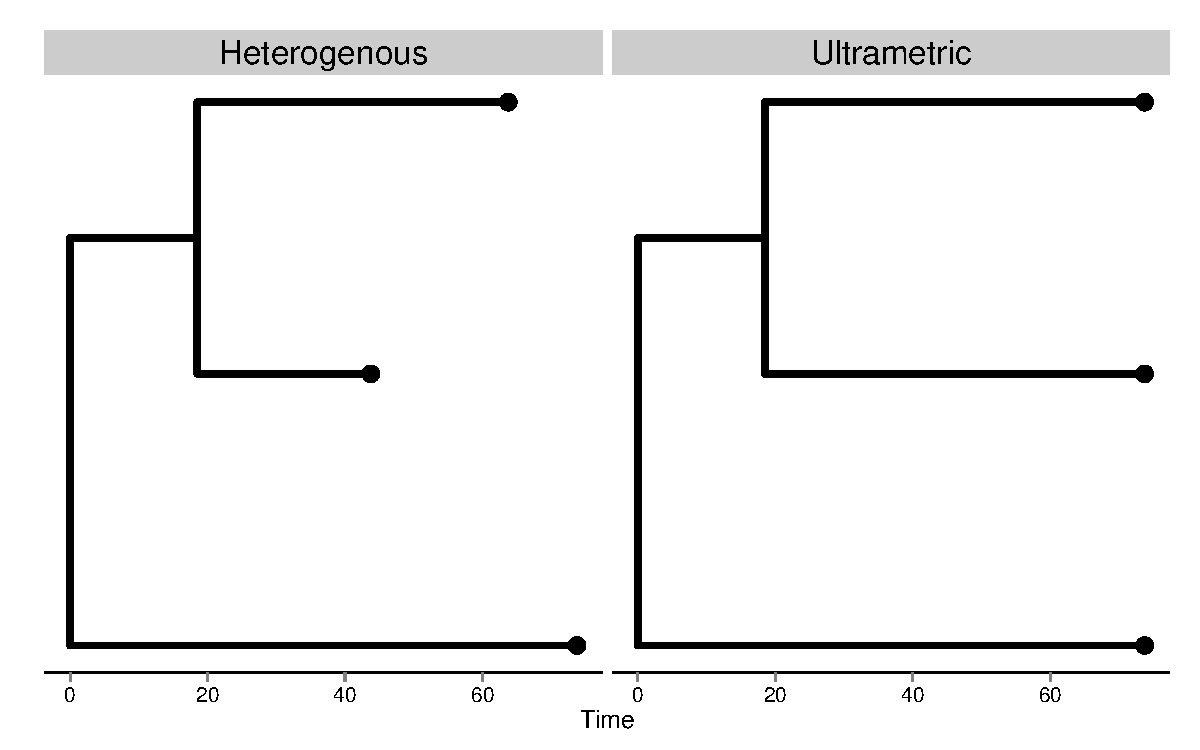
\includegraphics[scale=0.35]{ultrametric} 
\caption{
{ \footnotesize 
{\bf Different sampling schemes.} Tree on the right has all of it's sampling dates set at $t=0$. Conversly the tree on the left is sampled at different points in time and provides temporal information.
}% END: footnotesize
}
\label{fig:ultrametric}
\end{figure}

Such time stamped data-sets are usually reffered to as time-heterogeneous and frequently arise from studies involving viruses which accumulate statistically significant amounts of genetic change in a relatively short amount of time.
Populations for which such data can be obtained are called measurably evolving populations (MEPs, \cite{Drummond2003}) and have been instrumental in providing estimates of the evolutionary rate and in making advances to the theory of molecular clock models \citep{Drummond2006}.

In studies known as phylodynamics the processes which shape the viral genome are integrated with epidemiological dynamics, by assuming that both the evolution and 
geographical dispersal are independent, stochastic processes which unfold on phylogenetic trees.
In that sense the tree does not only provide a record of evolutionary ancestry, but also of the dispersal in actual geographical coordinates, and both these processes happen simultaneously.

Our group has been involved in research which aims at developing a full quantitative understanding of the processes that shape the epidemiology and the evolution of MEP-like viruses.
In the following section, I present the problems on which my involvement in this fascinating area of research has been focused.


\subsection{Processes Giving Rise to Genealogies: Demography and Migration}


[PL: Discuss variable size coalescent (demographic) models (which are the tree priors in BEAST)
Introduce phylogeography -- discrete ancestral state reconstruction is only one way of doing this (see Bloomquist, Lemey, Suchard)]


\subsection{Bayesian evolutionary inference in BEAST}


[PL: How this all integrates in a flexible framework and publicly available software, one that adequately accounts for phylogenetic uncertainty by averaging over all plausible evolutionary histories for your data
If there is too little here to build a subsection, you can attach it to the previous subsection and call that 'Bayesian genealogical inference using BEAST'
]



\subsection{Objectives: model extension, simulation and visualisation}

% models
Phylogenetic analysis employing stochastic processes make strong restrictive assumptions regarding the underlying substitution process.
These assumptions are mainly considered to reduce the number of free parameters of the models and ease the already mentioned computational and mathematical tractability.
Unfortunately many of these assumptions hamper the application of the methods to the complex, real-world data-sets.
Relaxing some of these assumptions and development of more biologically plausibe models, able to grasp the complex nature of phylodynamic dispersal processes is one the aims of the presented thesis \citep{Bielejec2014a}.
Another goal is to make the general applicability suitable for epidemiological problems as well as beyond them, with potential to turn the findings into usefull predictions of the emergence of infectious diseases, e.g. by identifying the sources and sinks of the viral spread.
% geographical dispersal

% simuation
With the development of novel phylogenetic inference methods comes the need to synthesize evolutionary data, in order to compare estimator performance and characterize strengths and weaknesses of different approaches (e.g. \cite{Arenas2012}, \cite{Hoban2011}).
Whereas the true underlying evolutionary relationships between biological sequences are generally unknown, Monte Carlo simulations allow generating test scenarios while controlling for the evolutionary history as well as the tempo and mode of evolution. 
Part of the research presented in this thesis is devoted towards development of a flexible software for sequence simulation, that integrates both the tree-generative processes, as well as models responsible for shaping the molecular histories and geographical dispersal \citep{Bielejec2014a}.

% visualisation
Phylogenetic inference inevitably results in complex, multi-dimensional output data.
This dimensionality is further incremented by adding the geography to the usuall evolutionary time component.
Finally, Bayesian analysis result in posterior distributions of trees, with each tree branch annotated with estimated node locations and other traits of interest.
These aspects represent a major challenge for visualizing the phylogenetic inference.
Yet clear and intuitive visualizations are an important aspect of every analysis \citep{Hadley2010}.

Spatial phylogenetic projections have already been utilized in the field \citep{Kidd2006,Parks2009}, yet most of these applications remain limited to mapping phylogenetic tip taxa to their geographical coordinates, without providing robust statistical estimates of the geographic locations at the ancestral nodes nor the measures of uncertainty in the inference.
Fortunately the advent of powerful and flexible Geographic Information Systems (GIS) has fostered an interesting possibility to incorporate both spatial and temporal information into viral phylogenetic analysis.

\begin{figure}[H]
\centering
\includegraphics[scale=0.3]{figures/spread}
\caption{
{ \footnotesize 
{\bf Phylogeographic visualization of viral spread in time and space.} 
A. Conceptual representation of time-slicing a phylogeny and projecting the part of the tree up to time $t_{1}$ and $t_{2}$ respectively. B. An example projection of influenza H5N1 over time in Google Earth for two different segment phylogenies. % (hemagglutinin and neuraminidase in green and magenta respectively).
} % END: footnotesize
}
\label{fig:spread}
\end{figure}

Presenting readily interpretable visual summaries of the inferences, that can in turn be communicated to the researchers across different fields is one of the more important aspects of this thesis.
This goal has been materialized in the development of a user-friendly application, that produces compelling and informative statistical visualizations of viral spread in time and space \citep{Bielejec2011}.
An example of such a visualisation finds itself in Figure~\ref{fig:spread}.

\section{Evolution as a stochastic process}

In order to provide a formal basis for the work in the research chapters of this thesis, this chapter proceeds with a description of general stochastic models of character substitution processes in phylogenies. 
Molecular phylogenetic modeling typically starts with an assumption that the observed sequence data has been generated by some stochastic process, which emits characters over time.
We can think of these stochastic processes as functions of time, which is regarded as a deterministic argument, whose values are random (non-deterministic) variables. 
It is thus a statistical model of a random development, or evolution, in time.
Phylogenetic inference often resorts to processes where time is considered to be continuous and the indexed set of outcomes, called the state space, is countable and finite (discrete).
% The stochastic process $X$ is a collection $\left\{ X(t):\; t\in T\right\} $, where each drawn value $X(t)$ is a random variable drawn from state space $\mathcal{E}$, with $K$ possible values, indexed by orderer time $T$.
With that in mind we can provide a formal definition:

\begin{definition} 
The stochastic process $X$ is a collection $\left\{ X(t):\; t\in T\right\} $, where each drawn value $X(t)$ is a random variable drawn from state space $\mathcal{E}$, with $K$ possible values, indexed by orderer time $T$.
\label{def:stochasticProc}
\end{definition} 

In the simplest case, for which the unit of evolution is a single nucleotide, we have $\mathcal{E}=\left\{ A,C,G,T\right\}$ and $K=4$.
The particular sites of the sequence alignment are then considered to be stochastically independent realizations of the process $X$, leading to the observed data (see Figure~\ref{fig:alignment}). 

\begin{figure}[H]
\centering
\begingroup
\everymath{\displaystyle}
{\Large
\begin{displaymath} % 
    \xymatrix@R+1pc{ 
\color{gray2}A \ar[r] & \color{gray2}T \ar[r] & A \\
\color{gray2}A \ar[r] & \color{gray2}T \ar[r] & G \\
\color{gray2}A  \ar[rr]_{ \color{gray2}\begin{array}{c}
A\rightarrow G\\
G\rightarrow C
\end{array}} &&  C
    } % 
\end{displaymath}
}% END: Large
\endgroup
\caption{
{ \footnotesize 
{\bf Evolution at a single site.} Over time characters at the site change, leading to the observed data (black). Some of the mutations may be silent. Each site evolves independently.
}% END: footnotesize
}
\label{fig:alignment}
\end{figure}

As Figure~\ref{fig:alignment} depicts not all of the differences can be observed, as due to multiple substitutions (multiple hits) some of the changes are silent.
%PL: better not use silent as this also used for 'non synonymous substitutions'
To accurately describe these processes one needs a models of evolution that can account for those multiple hits.
%PL: you need to state the obvious here: because of multiple hits, observed differences in the sampled genetic data will underestimate the underlying genetic distance, and this is what we can to account for using models.

\subsection{The Poisson process\label{sub:poisson}}

The Poisson process is an example of a continuous-time stochastic process that is frequently used to describe counts of independent, rare events, occurring with some intensity (or rate) $r$, that remains constant over time. 
Examples of such a process are the requests for a single document on a web-server, or the goals scored in a football game \footnote{Unless it's Real - Barca, than the events are not so rare.}.%PL or Brazil - Germany...
%The state space in this case is obviously $\mathcal{E} = \left\{ 0,1,2, \dots \right\}$.
The Poisson process is equally suitable to model the number and waiting times of DNA mutation of sequence substitution events. 
We can formally define a Poisson process as following:

\begin{definition} 
A Poisson process with rate $r>0$ is continuous-time counting process $\left\{ N(t):\; t\geq0\right\}$ such that:

\begin{itemize}
\item $N(0)=0$.
\item The increments are independent i.e. if $(t_{1},t_{2}]\cap(t_{3},t_{4}]=\emptyset$ then $N(t_2)-N(t_1)$ and $N(t_4)-N(t_3)$ are independent and stationary (i.e. the probability distribution of the number of occurrences counted in any time interval only depends on the length of that interval).
\item The number of events in any interval of length $t$ is $\text{Poisson}(r t)$.
\end{itemize}

Figure~\ref{fig:poisson} shows a sample of different trajectories of such a process.

\label{def:poisson}
\end{definition}

\begin{figure}[H]
\centering
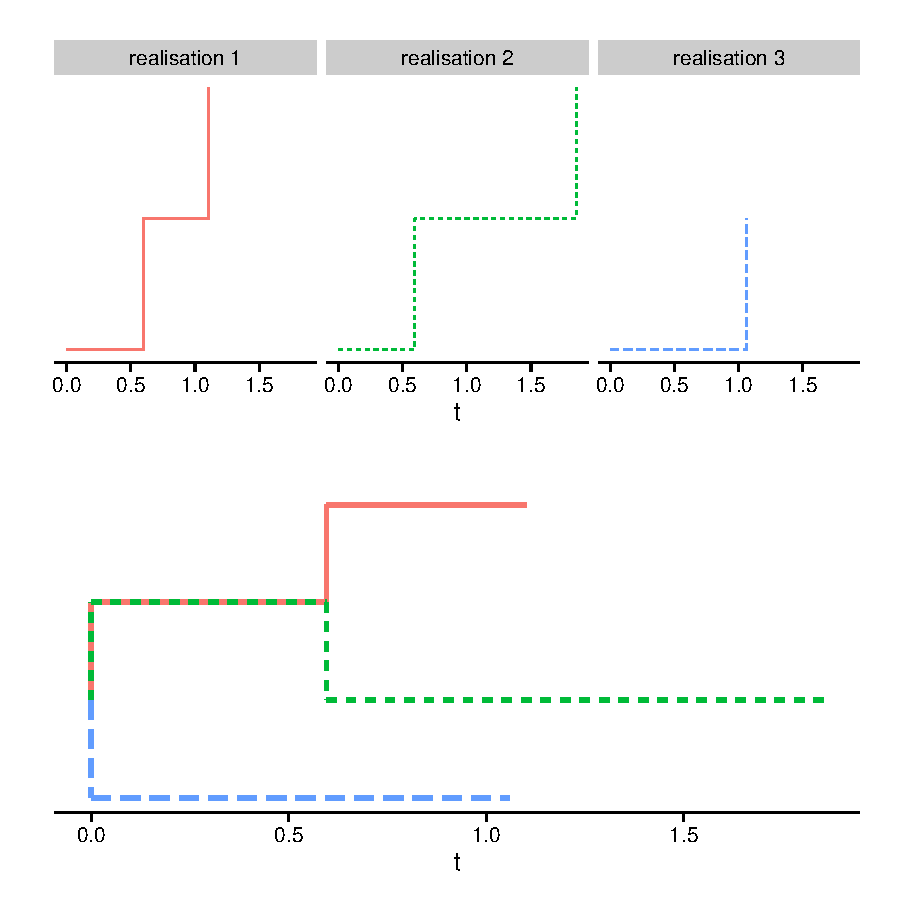
\includegraphics[scale=0.5]{poisson}
\caption{
{ \footnotesize 
{\bf Independent realizations of the Poisson process with intensity $r=1$.}
Times between mutations (the branch lengths) are \emph{iid} exponentially distributed random variables with mean $1/r$.
} % END: footnotesize
}
\label{fig:poisson}
\end{figure}

Let's assume that evolution at a single site is governed by a Poisson process $N$ with some intensity $r$.
Definition~\ref{def:poisson} implies that under this model the number of mutations $N(t+u)-N(u)$ in some time interval $(u,t+u]$ of length $t$ follows a Poisson distribution with expected number of events $r t$.
Thus we can write:

\begin{equation}
P\left\{ N(t+u)-N(u)=k\right\} =P\left\{ N(t)=k\right\}=\frac{e^{-r t}(r t)^{k}}{k!},\; k=0,1,\ldots
\label{eq:poissonDist} 
\end{equation}

In the Poisson process the time between any two mutations is exponentially distributed with parameter $r$, thus the average waiting time between the occurrence of events is $1/r$.
To show this important property we can consider $T_1,T_2,\ldots$ to be the the inter-arrival times, where $T_k$ is the waiting times between the $(k-1)\text{'st}$ and $k\text{'th}$ mutation. 
Obviously, the number of mutations before some time $t>0$ is less than some integer $k>0$ if and only if the waiting time $T_k$ until the $k\text{'th}$ mutation is larger than $t$:

\begin{equation}
P\left(N(t)<k\right)=P\left(T_{k}>t\right).
\end{equation}

\noindent
For the first waiting time $T_1$ we have:

\begin{equation}
1-P\left(T_{1}>t\right)=1-P\left(N(t)<1\right)=1-P\left(N(t)=0\right).
\end{equation}

\noindent
From Equation~(\ref{eq:poissonDist}) we have that:

\begin{equation}
F_{T_{1}}(t)=1-P\left(T_{1}>t\right)=1-e^{-r t},
\end{equation}

\noindent
therefore $T_1$ follows the exponential distribution with parameter $r$.
For the second waiting time $T_2$ and some arbitrary $u>0$ and $t>0$, the independent increments property implies that:

\begin{eqnarray}
F_{T_{2}}(t) &=& 1-P\left(T_{2}>t|T_{1}=u\right) \\ \nonumber
& = & 1-P\left(\text{no mutations in }(u,t+u]|T_{1}=u\right) \\ \nonumber 
& = & 1-P\left(N(t)=0\right)=1-e^{-r t}.
\end{eqnarray}

\noindent
Therefore $T_2$ is independent of $T_1$ and $\text{Exponential}(r)$. 
Similarly we can show that $T_3$ is independent of $T_1$ and $T_2$ and by repeating the same argument $T_1,T_2,\ldots$ are independent and identically distributed (i.i.d.) $\text{Exponential}(r)$ random variables.

% TODO: memoryless property does not depend at all, vide poiss)
% TODO: markovian (depends only a little)
% * difference? Memoryless is more

\subsection{Instantaneous rates of mutation\label{sub:rates}}

Within a phylogenetic framework the interest typically lies not only in modeling the number of events (mutations), but also the actual probabilities of changing states at the particular site in the alignment. 
We therefore need to generalize the process to a finite number of discrete states.
Let $\mathbf{R}$ denote a $K \times K$ matrix filled with probabilities of exchanging states between any pair $i,j\in \mathcal{E}$.
To express the probability of going from state $i$ to $j$ in some time interval $t$, we multiply the probability of the state change by the probability of having exactly $k$ events leading to the observed change, and integrate over all possible values of $k$.
This allows us to accommodate all possible paths that evolution might have taken, and to account for multiple hits that might have occurred at the site, as illustrated in Figure~\ref{fig:alignment}.
From Equation~(\ref{eq:poissonDist}) we know the probability of having $k$ mutations in time interval $t$, thus:

\begin{equation}
\left\{ P(t)\right\} _{ij}=\underset{k=0}{\overset{\infty}{\sum}}\mathbf{R}^{k}\frac{(r t)^{k}}{k!}e^{-r t}=\underset{k=0}{\overset{\infty}{\sum}}\frac{(\mathbf{R}r t)^{k}}{k!}e^{-r t},
\label{eq:matrixExp1}
\end{equation}

\noindent
where $\left\{ P(t)\right\} _{ij}$ denotes the $ij\text{-th}$ element of the transition probability matrix $\mathbf{P}$ over time $t \geq 0$.
Let us denote the matrix $\mathbf{R}-\mathbf{I}$, where $\mathbf{I}$ is a $K \times K$ identity matrix, by $\mathbf{Q}$.
Using the power series definition of the transition probability matrix $\exp(\mathbf{R})=\underset{k=0}{\overset{\infty}{\sum}}\mathbf{R}^{k}/k!$ we can write Equation~(\ref{eq:matrixExp1}) as:

\begin{equation}
\left\{ P(t)\right\} _{ij}=e^{\mathbf{R}r t}e^{-r t} =e^{(\mathbf{R}-\mathbf{I})r t}=e^{\mathbf{Q}r t} 
\label{eq:matrixExp2}
\end{equation}

\noindent
Single entry $q_{ij} \ge 0$ for $i \neq j$ in matrix $\mathbf{Q}$ quantifies the probability of changing from state $i$ to $j$ in an infinitely small amount of time, therefore we will refer to $\mathbf{Q}$ as the \emph{instantaneous rate matrix}.

\subsection{Computing the matrix exponent \label{sub:exponentiation}}

In order to arrive at the finite-time transition probabilities matrix $\mathbf{P}(t)$ for some time $t\geq0$ one needs to compute the matrix exponential in Equation~\ref{eq:matrixExp2}.
\cite{Moler1978} provide an excellent review of numerical methods to compute the matrix exponent. 
Here we will highlight the method utilized by most phylogenetic software, including BEAGLE \citep{Ayres2012} and BEAST \citep{Drummond2012}, that uses the singular value decomposition (SVD) of the rate matrix $\mathbf{Q}$.   

Let us assume $\mathbf{Q}$ has $K$ linearly independent eigenvectors $\mathbf{v}_{i} \; (i=1,\ldots,K)$ with corresponding eigenvalues $\lambda_{i}\;(i=1,\ldots,K)$:

\begin{equation}
\mathbf{Q}\times\mathbf{V}=\lambda\times\mathbf{V}
\label{eq:eigenvaluesEigenvectors}
\end{equation}

\noindent
This condition is sufficient for $\mathbf{Q}$ to be diagonizable, thus it's Jordan form is:

\begin{equation}
\mathbf{V}\times\mathbf{Q}\times\mathbf{V}^{-1}=\left[\begin{array}{cccc}
\lambda_{1} & 0 & \cdots & 0\\
0 & \lambda_{2} & \ddots & \vdots\\
\vdots & \ddots & \ddots & 0\\
0 & \cdots & 0 & \lambda_{K}
\end{array}\right]=\text{diag}(\lambda_{1},\ldots,\lambda_{K})=\mathbf{D} ,
\label{eq:diagonalization}
\end{equation}

\noindent where $\mathbf{V}$ is a matrix composed of eigenvectors of $\mathbf{Q}$. 
Multiplying both sides of Equation~(\ref{eq:diagonalization}) with the edge length $t$ and scaling by the appropriate rate scalar $r$, we can write $\mathbf{Q}$ in the following form:

\begin{equation}
rt\mathbf{Q}=\mathbf{V}\times\text{diag}(rt\lambda_{1},\ldots,rt\lambda_{K})\times\mathbf{V}^{-1} .
\end{equation}

\noindent Finally, using the power series definition of the transition probability matrix, we obtain: 

\begin{eqnarray}
\mathbf{P}(t) & = & \exp\left(rt\mathbf{Q}\right)  =  \underset{k=0}{\overset{\infty}{\sum}}\left(rt\mathbf{Q}\right)^{k}/k! 
 =  \underset{k=0}{\overset{\infty}{\sum}}\left(\mathbf{V}\times\mathbf{D}\times\mathbf{V}^{-1}\right)^{k}/k! \\ \nonumber
& = & \mathbf{V}\times\left(\underset{k=0}{\overset{\infty}{\sum}}\mathbf{D}^{k}/k!\right)\times\mathbf{V}^{-1} = \mathbf{V}\times\text{diag}(e^{rt\lambda_{1}},\ldots,e^{rt\lambda_{K}})\times\mathbf{V}^{-1} ,
\label{eq:eigen_decomposition}
\end{eqnarray}

\noindent 
where the last transition is due to the fact that the exponential of the diagonal matrix is obtained by exponentiating every entry on the main diagonal.
We should note here that the repeated evaluations of $\exp\left(rt\mathbf{Q}\right)$ for different times $t$ are all based on the same SVD of the matrix $\mathbf{Q}$. 
One needs only to scale and exponentiate the eigenvalues to calculate the diagonal matrix $D$ and perform two matrix multiplications, thus reducing all calculations to a simple and effective algorithm. 

\subsection{Markov chain models of sequence substitution\label{sub:subst_models}}

% TODO markov property is inherited from Poisson process
Drawing realizations with probabilities defined by $\mathbf{P}$  gives rise to a continuous-time stochastic process $\left\{ X(t):\; t\geq0\right\}$ satisfying the Markov property, such that for every $n\geq 0$, given the time points $0\leq t_{0}\leq t_{1}<\ldots<t_{n}\leq t_{n+1}$ and discrete states $i_{0},i_{1}, \ldots, i_{n},i_{n+1}$ it holds that: 

\begin{eqnarray}
P\left\{ X(t_{n+1})=i_{n+1}\mid X(t_{n})=i_{n},\ldots, X(t_{0})=i_{0}\right\} & = & \\ \nonumber
P\left\{ X(t_{n+1})=i_{n+1}\mid X(t_{n})=i_{n}\right\} .
\label{eq:markov}
\end{eqnarray}

The elements of $\mathbf{P}$ quantify the finite-time transition probabilities between the $K$ discrete state-space elements.
This describes a Continuous-time Markov chain (CTMC), which  we will use to model the substitution process at a single site of an alignment.
Every CTMC is completely characterized by its rate matrix $\mathbf{Q}$ and the stochastic matrix $\mathbf{P}(t),\ t\geq0$ is obtained via matrix exponentiation as described in the previous subsection (Subsection~\ref{sub:exponentiation}).

%---SUBSTITUTION MODEL---%
\begin{figure}[H]
\centering
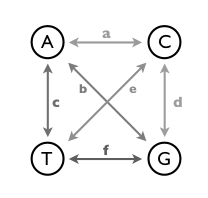
\includegraphics[scale=0.5]{substitution} 
\caption{
{ \footnotesize 
{\bf  Graphical representation of  a nucleotide substitution model.} A Markov substitution model with a symmetrical matrix.
} % END: footnotesize
}
\label{fig:substitution}
\end{figure}

Figure~\ref{fig:substitution} depicts an example of such a CTMC substitution model, governing the substitution rates between four discrete nucleotides, where all the pairs communicate (all states have a non-zero transitional probability of exiting from, i.e. all states are non-absorbing).
Let us denote a transition probability between two states $i$ and $j$ over time $u$ to $t+u$ by:

\begin{equation}
p_{ij}\left(u,t+u\right)=P\left\{ X(t+u)=j\mid X(u)=i\right\} .
\end{equation}

In the phylogenetic setting, researchers often constrain the CTMC processes, mostly for computational and mathematical convenience.
A frequently applied restriction is to assume time-homogeneity of the substitution process, which states that the evolution does not change in pattern over time, and therefore transition probabilities depend only on the time difference $t$ between $u$ and $t + u$:

\begin{equation}
p_{ij}\left(t\right) = p_{ij}\left(0,t\right) = p_{ij}\left(u,t+u\right).
\label{eq:time_homogeneity}
\end{equation}

Unfortunately this assumption does not hold for many real-world data-sets and precludes the identification of biologically interesting patterns in the evolutionary process. %, as the temporal dynamics clearly do shift in time, often in a seasonal, observable manner \citep{Bahl2011}.
%PL: deleted the above subsentence as it is too specific to phylogeography
One of the goals of the research presented in this thesis is to efficiently confront situations in which this assumption does not hold.
% can grasp such situations.

Substitution models are further constructed to be ergodic, meaning that there exist positive values $\pi_{1},\pi_{2},\ldots,\pi_{K}$ such that:

\begin{equation}
\forall i,j\in \mathcal{E}  \quad\underset{t\rightarrow\infty}{lim}p_{ij}(t)=\pi_{j}.
\label{eq:ergodicity}
\end{equation}

% $\mathbf{\Pi}$

As $t$ goes to infinity the probability that the site is in some state $j$ is non-zero and does not depend on the starting state $i$.
This implies that the chain will always display the same long-term behavior, which is why $\mathbf{\Pi}=\{\pi_{i},\ i\in\mathcal{E}\}$ is called a \emph{stationary distribution} (also referred to as the \emph{equilibrium distribution} or \emph{equilibrium frequencies}).
We can look at the elements of $\mathbf{\Pi}$ as the proportion of time spent in state $j\in\mathcal{E}$ after the Markov chain has run for infinitely long time, that does not depend upon the initial state $i$ of the process.
In other words if we sample the initial state from the stationary distribution and then let the process run for some sufficiently long time $t$, then the distribution of the final state will equal the stationary distribution. 

Another commonly applied constraint is that of \emph{time-reversibility}, meaning that the model does not care which character is the ancestor and which is the descendant so long as all other parameters are held constant.
For all $i,j\in \mathcal{E}$ and $t\geq 0$ we have:

\begin{equation}
\pi_{i}p_{ij}(t)=\pi_{j}p_{ji}(t).
\label{eq:time_reversibility1}
\end{equation}

\noindent
Condition~\ref{eq:time_reversibility1} is also referred to as the \emph{detailed balance} equation, and posits that the probability of sampling $i$ from the stationary distribution and then going to $j$ over some finite-time $t$ is the same as sampling $j$ and going to $i$. 
% By the definition of $\mathbf{\Pi}$ and $\mathbf{P}$ from (\ref{eq:time_reversibility1}) we have:
% 
% \begin{equation}
% \pi_{i}q_{ij}=\pi_{j}q_{ji}\mathbf{Q}.
% \label{eq:time_reversibility2}
% \end{equation}
% 
% Definition (\ref{eq:time_reversibility1}) and (\ref{eq:time_reversibility2}) are equivalent.
This condition is assumed for strictly computational reasons, i.e. time-reversibility makes it easier to diagonalize $\mathbf{Q}$, which - as we have described in 
Subsection~\ref{sub:exponentiation} - is a strategy frequently employed in phylogenetic software to compute the exponentials of rate matrices.
Time reversibility also simplifies the computation of the likelihood on a tree, since it makes the computation indifferent to the position of the root, which we will discuss in Subsection~\ref{sub:likelihood}.

%TODO: JK69 as example
\subsection{A simple example: the Jukes and Cantor substitution model\label{sub:jc69}}

In this subsection we will discuss the simplest model of nucleotide substitution, i.e. the JC69 model \citep{Jukes1969}.
The JC69 model assumes that the instantaneous rates of change between every two nucleotides are the same.
We also require that the rate matrix $Q$ characterizing the model is a stochastic matrix (each row sums to 0).
The infinitestimal rate matrix of the JC69 model is thus given by:

\begin{equation}
\mathbf{Q}=\left[\begin{array}{cccc}
-3r & r & r & r\\
r & -3r & r & r\\
r & r & -3r & r\\
r & r & r & -3r.
\end{array}\right]
\label{eq:jc69}
\end{equation}

\noindent
The finite-time transition probability matrix $\mathbf{P}(t)$ for time $t>0$ is calculated using matrix exponentiation  (see Subsection~\ref{sub:exponentiation}):

\begin{equation}
\mathbf{P}\left(t\right)=\left[\begin{array}{cccc}
p_{0}(t) & p_{1}(t) & \cdots & p_{1}(t)\\
p_{1}(t) & p_{0}(t) & \ddots & \vdots\\
\vdots & \ddots & p_{0}(t) & p_{1}(t)\\
p_{1}(t) & \cdots & p_{1}(t) & p_{0}(t)
\end{array}\right],\text{ where }\ensuremath{\begin{cases}
p_{0}(t)=\frac{1}{4}+\frac{3}{4}e^{-4rt}\\
p_{1}(t)=\frac{1}{4}-\frac{1}{4}e^{-4rt}
\end{cases}}.
\label{eq:jc69Finite}
\end{equation}

\noindent
A few things are worth mentioning about Equation~(\ref{eq:jc69Finite}).
If we let $t\rightarrow \infty$ we can see that $\forall i,j\; p_{ij}(t)=1/4$, which means that the equilibrium distribution for the JC69 model is: 

\begin{equation}
\mathbf{\Pi}=\left\{ \pi_{T}=1/4,\pi_{C}=1/4,\pi_{A}=1/4,\pi_{G}=1/4\right\}
\label{eq:jc69Steady}
\end{equation}

\noindent
Second, the rate and time in Equation~(\ref{eq:jc69Finite}) occur as a product, which means that rate and time are confounded.
If we were to simulate two sequences, using the algorithm listed in (\ref{alg:simulation}) and starting the random number generators form the same seed, they will look the same for every $r$ and $t$ as long as their product $rt$ is the same.
This is true for most of the substitution models and implies that typical phylogenetic estimation focuses on inferring the product parameter $\theta=rt$ or genetic distance.
%PL: perhaps mention that the section on molecular clocks (cfr supra) discusses the conditions for which we can start separating time and rate

\subsection{Phylogenetic tree}

%PL: According to the extension I recommend for the general intro, a tree should already be introduced properly there, and this should from the biological perspective but can also include this more formal description..

A phylogenetic tree, or phylogeny for short, depicts the genealogical relationship between character sequences.
Mathematically, a phylogeny $\mathbf{F}$ represents a directed, acyclic graph with sets of \emph{nodes} connected by \emph{branches} (e.g., Figure~\ref{fig:treeconcept}).
Data is observed only at the external nodes (\emph{tips}), while internal nodes represent extinct ancestors for which data is usually missing.
The ancestor of all observed samples is called the \emph{root} of the tree and it's height is reffered to as the time to the most recent common ancestor (TMRCA).

%---TREE CONCEPT---%
\begin{figure}[H]
\centering
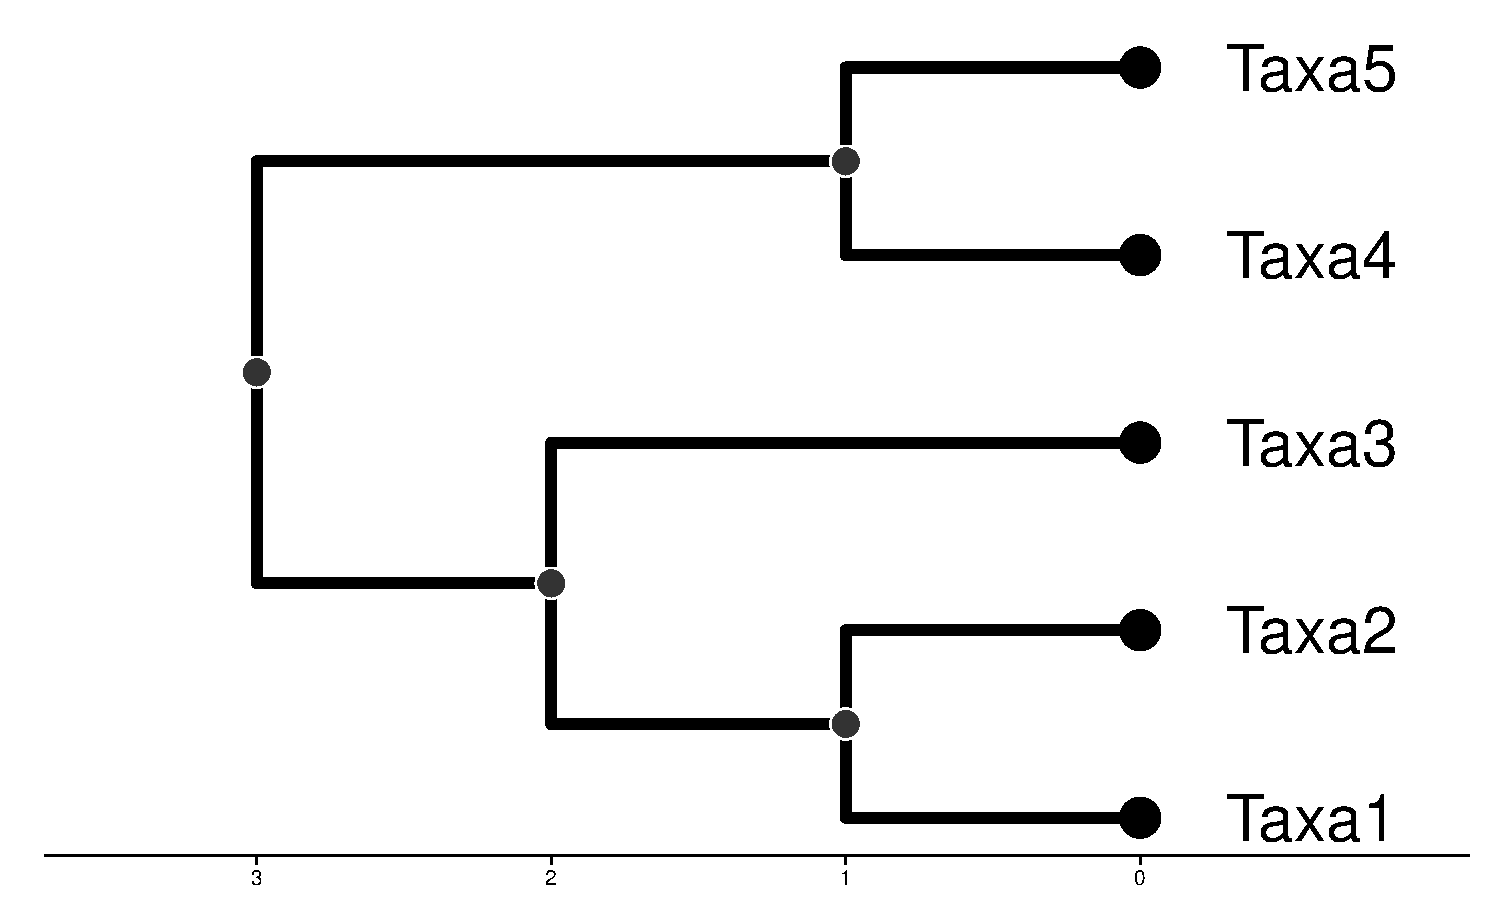
\includegraphics[scale=0.35]{treeconcept} 
\caption{
{ \footnotesize 
{\bf A phylogenetic tree showing evolutionary relationship.} Character sequences are observed at the tips of the tree (black dots); sequence characters at the internal nodes are treated as missing data. 
Branch lengths are estimated in units of genetic distance, or in this case, real time.
} % END: footnotesize
}
\label{fig:treeconcept}
\end{figure}

Within our framework we focus on trees which are rooted and time-measured, i.e. their branch lengths are scaled in actual time units.
A rooted binary tree with $n$ leaves has $2n-2$ branches and $n-1$ internal nodes.
The branching pattern of the tree is called the \emph{topology}. 

\subsection{Sequence evolution on a tree\label{sub:evolutionOnTree}}

In this section we proceed by describing the connection between the CTMC models of character substitution discussed above and phylogenetic histories.
We keep the focus on a single site of the alignment, and due to the assumption of independence the probability of observing an alignment is simply the product of probabilities for observing the individual sites.

To gain a better understanding of the process shaping the data observed at the tips of a phylogenetic tree let us consider the problem of simulating sequence evolution on a tree according to a model with rate matrix $\mathbf{Q}$.
We start with a first character $i$ sampled at the root of the tree $x_0$ from the stationary distribution $\mathbf{\Pi}$.
Let us assume that two direct descendent nodes are $x_j$ and $x_k$.
The character sampled at the root waits an exponentially distributed amount of time $t\geq0$ (see Figure~\ref{fig:poisson}) before moving to one of the descendent or child nodes.
Such traversal is said to be following the pre-order, i.e. parental nodes are visited before child nodes.   
The process then randomly decides by a coin flip to which of the two descendent nodes to move next (assuming that the visited node is not a tip).
Let us assume that the process moved to $x_j$.
The state $j$ for the node $x_j$ is sampled conditional on the value $i$ already sampled at the root using the branch length expressed in real time $t$ and the vector probabilities in the row $i$ of the finite-time probabilities matrix $\mathbf{P}(t)$, calculated using SVD of the rate matrix $\mathbf{Q}$ that characterizes the CTMC.   

\begin{algorithm}[H]
\centering
\begin{algorithmic}[1]
% \footnotesize{
%
\State $node \gets getRoot\left(\right)$
%
\State $state \gets getState\left(node\right)$
%
\Repeat
%
\If{$\left(hasChildren\left(node\right)\right)$}
%
\ForAll{children}
%
\State $t \gets getDistanceToParent\left(child\right);$
%
\State $ \mathbf{P}\left(t\right) \gets e^{\mathbf{Q}t};$
%
\State $state \gets sample\left(\mathbf{P}\left[ state, \right]\right);$
%
\EndFor
%
\Else \Comment{this is tip node}
%
\State $node \gets getParent\left(node\right);$
%
\EndIf
%
\Until{$\left(\text{simulated for all nodes}\right)$}
% }
\end{algorithmic}
\caption{
{ \footnotesize 
%PL: Perhaps add: Pseudo code for simulating...
{\bf Simulation an evolutionary process along a phylogeny.} 
When a child node is visited, the state is sampled with conditional probabilities of changing to state $j$ given state $i$ at the parental node.
}% END: footnotesize
}
\label{alg:simulation}
\end{algorithm}

This illustrates the Markov property of a CTMC, as defined in Equation~(\ref{eq:markov}).
The sampling is then repeated on the node $x_j$, before recursively proceeding to the other trio of nodes.
The states sampled at the tips of the tree constitute the character sequence for one site of the alignment.
In this light the CTMC process can be viewed as a continuous-time random-walk, unfolding on the topology $\mathbf{F}$, with its behaviour described by a rate-matrix $\mathbf{Q}$.
The complete algorithm is listed in Algorithm~\ref{alg:simulation}.

\section{Likelihood of sequence evolution}

\subsection{Calculation of the likelihood on a tree\label{sub:likelihood}}

Likelihood is defined as a conditional probability of observing the data given the parameters, as a function of those parameters.
Phylogenetic inference considers discrete molecular sequence data in the form of aligned matrix $\mathbf{X}$ of size $n \times l$, where $x_{jh}$ is the $h$-th character in $j$-th sequence.
Single column $\mathbf{x}_{h}$ of the data matrix constitutes a single site.
Again, the standard assumption of independence posits that different sites evolve independently and that once two branches split at a node, the evolution on those branches is also independent.

In Subsection~\ref{sub:evolutionOnTree} we described how evolution according to some process $\mathbf{Q}$ gives rise to the observed data $\mathbf{X}$.
In the typical situation we start with just the observed data and aim the inference efforts at modeling the process that generated the alignment.
We can therefore denote the likelihood simply as: 

\begin{equation}
L\left(\mathbf{\Theta}|\mathbf{X}\right)=P\left(\mathbf{\Theta}|\mathbf{X}\right), 
\label{eq:likelihood}
\end{equation}

\noindent
where $\mathbf{\Theta}$ is the topology, branch lengths, parameters of the substitution model and other parameters of interest that we aim at estimating.
This quantity expresses how likely it is to observe the data given a specific value of the parameter of interest $\mathbf{\Theta}$.
By finding the value of $\mathbf{\Theta}$ that maximizes (\ref{eq:likelihood}) we capture a model with the best possible fit.

In this thesis we will not discuss the maximum likelihood estimation itself, rather focus on closely related methods of Bayesian inference.
The likelihood is nontheless required for both frameworks, and it enters the Bayesian schema as the data component.
We will now discuss how to calculate the likelihood of observing a certain realised sequence of characters on the tips of a tree, given a substitution model with fixed parameters.

%---LIKELIHOOD---%
\begin{figure}[H]
\centering
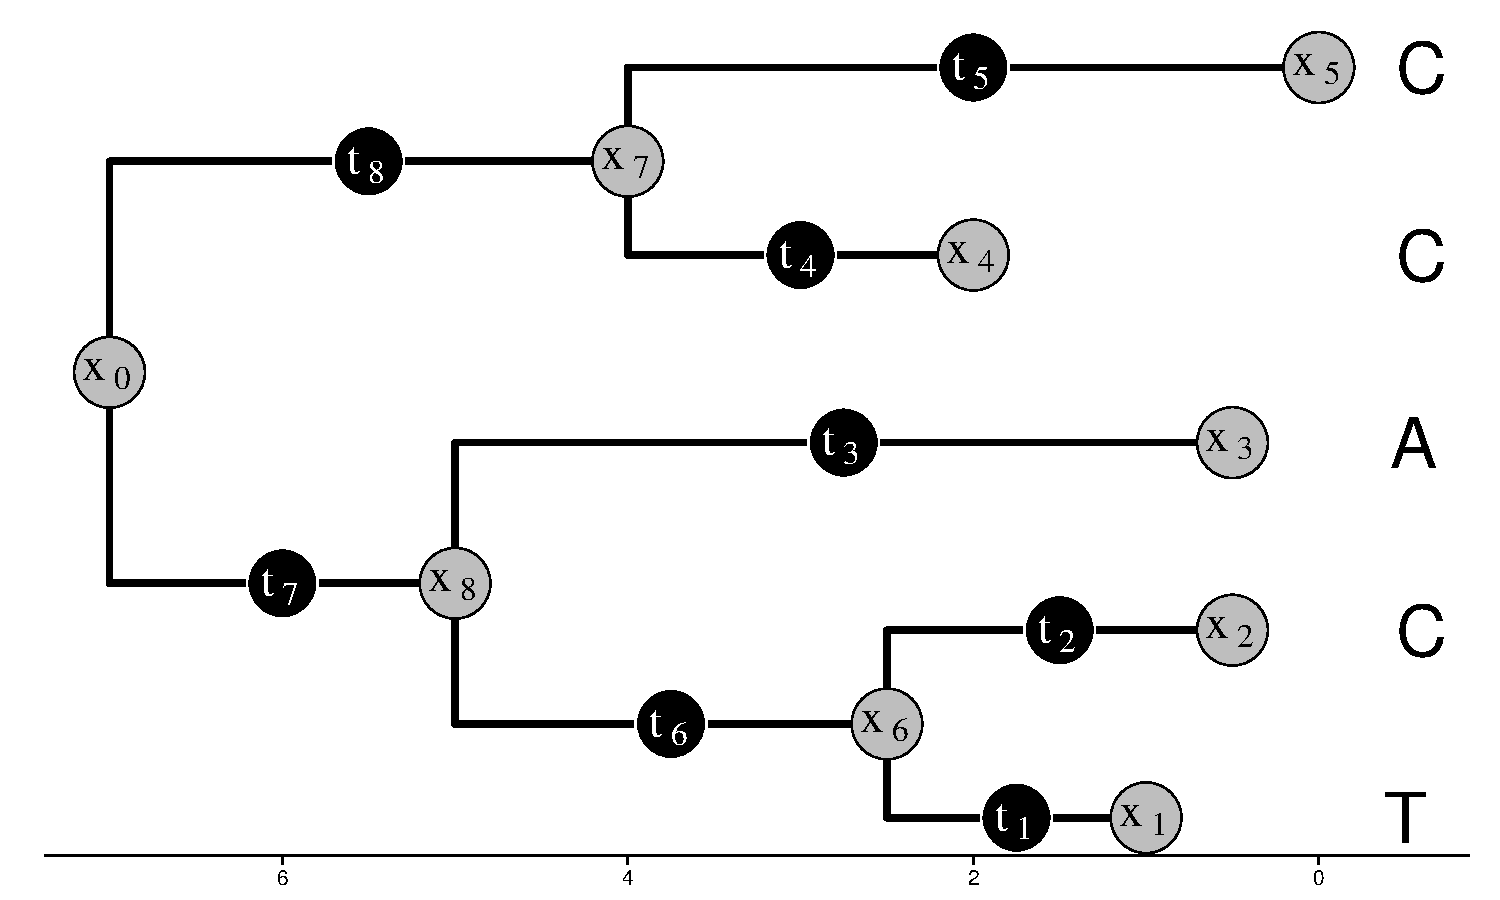
\includegraphics[scale=0.5]{likelihood} 
\caption{
{ \footnotesize 
{\bf  A tree with five taxa.} Character sequence data for single site is observed at the tips of the tree.
} % END: footnotesize
}
\label{fig:LIKELIHOOD}
\end{figure}

To calculate the likelihood means thus to reverse-engineer the evolution as it happened.
Figure~\ref{fig:LIKELIHOOD} presents single site with data $TCACC$ observed at the tips of the tree.
External nodes are numbered $x_{1}, \ldots x_{5}$, internal nodes $x_{6}, \ldots x_{8}$ and the root is placed at the node $x_{0}$.
Length of each branches leading to node $i$ is denoted as $t_{i}$.
Using methods presented in Subsection~\ref{sub:exponentiation} we calculate the finite-time transition probabilities $p_{ij}(t_{i})$ between all pairs of characters in the alignment.
According to the independence assumptions to calculate the probability at a single site we need to sum over all possible combinations that could give rise to the observed sequence. Thus:

\begin{eqnarray}
\underset{x_{0}\in \mathcal{E}}{\sum}\;\underset{x_{6}\in \mathcal{E}}{\sum}\;\underset{x_{7}\in \mathcal{E}}{\sum}\;\underset{x_{8}\in \mathcal{E}}{\sum}[\pi_{x_{0}}\cdot p_{x_{0}x_{8}}(t_{7})\cdot p_{x_{0}x_{7}}(t_{8})\cdot p_{x_{8}x_{6}}(t_{6})\cdot p_{x_{8}A}(t_{3}) \cdot \\ \nonumber
p_{x_{7}C}(t_{4})\cdot p_{x_{7}C}(t_{5})\cdot p_{x_{6}T}(t_{1})\cdot p_{x_{6}C}(t_{2})]
\label{eq:likelihoodNaive}
\end{eqnarray}

We can break down the terms in Equation~(\ref{eq:likelihoodNaive}) to the probability of observing the data $TCACC$ for the tips and $x_{0},x_{6},x_{7},x_{8}$ for the ancestral nodes (inside the brackets) and the sum over all possible path combinations over the state space $\mathcal{E}$ (outside the brackets).
Term $\pi_{0}$ is simply the probability that the root has character $x_{0}$ and comes from the assumption that the process generating the data has reached its equilibrium.

Summing over all possible paths leading to the observed data is computationally expensive, as there are  $K^{n-1}$ possible combinations, where $n-1$ is the number of internal nodes of a rooted binary tree.
Fortunately we can used the assumption of independence of the process in the two sub-trees below every node.
\citet{Felsenstein1981} provides an efficient algorithm for computing the likelihood of observing the data on a topology $\mathbf{F}$ given the substitution model that quantifies transition probabilities.
This routine, known as \emph{tree pruning} conveniently expresses the partial likelihood $L_{i}(x_{i})$ of observing data at the descendant tips of node $i$ given state $x_{i}$ at node $i$ in terms of partial likelihoods at nodes $j$ and $k$.
For all internal nodes of $\mathbf{F}$ we have:

\begin{equation}
L_{i}(x_{i})=\left[\underset{x_{j}\in \mathcal{E}}{\sum}\mathbf{P}_{x_{i}x_{j}}(t_{j})L_{j}(x_{j})\right]\times\left[\underset{x_{k}\in \mathcal{E}}{\sum}\mathbf{P}_{x_{i}x_{k}}(t_{k})L_{k}(x_{k})\right]
\label{eq:felsenstein1}
\end{equation}

\noindent
For tip nodes we have:

\begin{equation}
L_{i}(x_{i})=\begin{cases}
1 & \text{if }\hat{x}(i)=x_{i}\\
0 & \text{otherwise}
\end{cases},
\label{eq:felsenstein2}
\end{equation}

\noindent
where $\hat{x}(i)$ denotes the character state observed at node $i$.
After recursively applying (\ref{eq:felsenstein1}) to all the nodes of $\mathbf{F}$ in post-order fashion the likelihood of the data at the site is given by:
% we can integrate out the unobserved states calculating successive contributions to the partial likelihood.

\begin{equation}
L(\mathbf{x}_{h})=\underset{x_{0}\in\mathcal{E}}{\sum}\pi_{x_{0}}\cdot L_{0}(x_{0})
\label{eq:felsenstein3}
\end{equation}

\noindent
The log-likelihood of the whole alignment $X$ is computed by summing the logarithms of the likelihoods at the particular sites, due to the assumption of their independence:

\begin{equation}
l(X)=\underset{j=1}{\overset{l}{\sum}}log\left(L(\mathbf{x}_{jh})\right)
\label{eq:loglikelihood}
\end{equation}

\subsection{Computational burden of the likelihood computation}

We have already mentioned that the run-time of phylogenetic analysis is the caveat, hampering the development and application of novel, more biologically plausible methods in the field.
These limits are being actively stretched, mostly by porting the computationally expensive calculations to high-performance parallel devices such as Graphics-Processing Units (GPUs, \cite{Nickolls2008}).
In Subsection~\ref{sub:exponentiation} we already discussed how the computation of finite-time transition probabilities can be reduced to simple matrix algebra operations, which can than be ported to high-performance libraries and APIs for statistical phylogenetics such as the BEAGLE library \citep{Ayres2012, Suchard2009}. 

Before we proceed to discussing the burden imposed by certain steps when calculating the likelihood of a sequence evolution on a tree we need a formal definition of the computational complexity of a sequential routine.
Efficiency of an algorithm can depend on various factors, like network usage, disk usage, operational memory usage or CPU real-time usage.
All of these factors should be taken into consideration when designing and implementing a computational routine, however for most of the calculations the latter, i.e. CPU time will be the rate-limiting factor.
Typically both mathematicians and computer scientists use the Big-O notation as a relative representation of the algorithms complexity, like the execution time required.
Here we give a formal definition of the Big-O notation:

\begin{definition}
Let us assume two functions $f:\mathbb{R}_{>0}\rightarrow\mathbb{R}_{>0}$ and $T:\mathbb{R}_{>0}\rightarrow\mathbb{R}_{>0}$. 
For $n \in \mathbb{R}_{>0}$ we write:

\begin{equation}
T(n) \in \mathcal{O}\left(f(n)\right)
\label{eq:bigOh}
\end{equation}

\noindent
if and only if there exists constant $M>0$ and some $n_0 \in \mathbb{R}_{>0}$ such that:

\begin{equation}
T(n)\leq M \cdot f(n)
\end{equation}
\end{definition}


% \noindent
In other words $T(n)$ is $\mathcal{O}\left(f(n)\right)$ if and only if for all sufficiently large input values $T(n)$ is bounded from above by some constant multiple of $f(n)$.
This makes the Big-O notation useful when analysing algorithms for run-time efficiency and makes it possible to for example compare routines without the added overhead of neglectable terms, such as the architecture at which the code was run, the choice of language or compiler.
We will now briefly discuss some of the most common serial computational orders and their examples. 

\begin{algorithm}[H]
\centering
\begin{algorithmic}[1]
% \footnotesize{
\State $a \gets \text{\textbf{new int}}$;
%
\If{ $\left(a == 1 \right)$ }
%
\State \textbf{return} $true$;
%
\Else 
%
\State \textbf{return} $false$;
%
\EndIf
% }
\end{algorithmic}
\caption{
{ \footnotesize 
{\bf Single test operation.} 
} % END: footnotesize
}
\label{alg:o1}
\end{algorithm}

The simplest, most basic example is an operation that takes the same amount of time every time it is called, thus requiring constant time, i.e. it's computational complexity is that of $\mathcal{O}\left(1\right)$ and does not depend on the input size.
An example of such routine is listed in the Algorithm~\ref{alg:o1} that checks for a specific value of a constant.

\begin{algorithm}[H]
\centering
\begin{algorithmic}[1]
% \footnotesize{
\State $a \gets \text{\textbf{new int}}\left[n\right]$;
%
\For{int $\left(i=0; \; i<a.size(); \; i++\right)$}
%
\If{ $\left(a\left[i\right] == 1 \right)$ }
%
\State \textbf{return} $true$;
%
\Else 
%
\State \textbf{return} $false$;
%
\EndIf
%
\EndFor
% }
\end{algorithmic}
\caption{
{ \footnotesize 
{\bf Search for a value.} 
}% END: footnotesize
}
\label{alg:on}
\end{algorithm}

Algorithm which proceeds at $\mathcal{O}\left(N\right)$ has it's run-time growing linearly with the size of input data.
Example of such a routine is presented as Algorithm~\ref{alg:on}, which searches an array looking for a specific value.
We should note that the Big-O notation always describes the performance in worst-case scenario, i.e. a full loop has to be executed before a matching element is found, while for the actual real-world problem this does not have to be the case and the loop can return earlier.

\begin{algorithm}[H]
\centering
\begin{algorithmic}[1]
% \footnotesize{
\State $a \gets \text{\textbf{new int}}\left[n\right]$;
%
\For{int $\left(i=0; \; i<a.size(); \; i++\right)$}
%
\For{int $\left(j=0; \; j<a.size(); \; j++\right)$}
%
\If{ $\left(i == j \right)$ }
%
\State \textbf{do nothing};
%
\Else 
%
\If{ $a\left[ i \right] == a\left[ j \right]$ }
%
\State \textbf{return} $true$;
%
\EndIf
%
\EndIf \Comment{END: i == j check}
%
\EndFor \Comment{END: j loop}
%
\EndFor \Comment{END: i loop}
% }
\end{algorithmic}
\caption{
{ \footnotesize 
{\bf Search for a first duplicated value.} 
}% END: footnotesize
}
\label{alg:on2}
\end{algorithm}

An algorithm can also require a quadratic, $\mathcal{O}\left(N^2\right)$ run-time, i.e. it's performance is directly proportional to the square of the size of the input data.
Among examples of such an algorithm is the routine that searches for a duplicated value in an array, and requires two nested loops as presented in Algorithm~\ref{alg:on2}.
Similarly nesting more loops will result in routines which proceed at polynomial times $\mathcal{O}\left(N^3\right)$, $\mathcal{O}\left(N^4\right)$, $\mathcal{O}\left(N^5\right)$ etc.
An algorithm which proceeds at $\mathcal{O}\left(c^N\right)$, where $c>1$ is some constant, will have it's run-time growing c-times with every additional data element, i.e. exponentially. 

With those basic ideas described we can now come back to the original problem of calculating the likelihood of a sequence evolution on a fixed tree.
From Subsections \ref{sub:exponentiation} and \ref{sub:likelihood} we already know the steps involved:

% I skipped site rate variability, but perhaps it should be mentioned? 
\begin{enumerate}
\item { Singular value decomposition of the rate matrix $\mathbf{Q}$. }
\item { Taking the exponential of $\mathbf{Q}t$ for each branch length $t$. }
\item { Applying Equation~(\ref{eq:felsenstein1}) for every site in the alignment and every possible state in the state space $\mathcal{E}$. }
\item { Taking the logarithm and summing over all sites in the alignment. }
\end{enumerate}

Step (i) proceeds at ${\cal{O}}(K^3)$, however for typical, time-homogeneous applications this is not the a rate-limiting step, as repeated evaluations of $\exp(\mathbf{Q}t)$ in (ii) are based on the same decomposition of the matrix \citep{Suchard2009}. 
Step (ii) typically boils down to repeated matrix-vector-matrix multiplications and its serial computational order is ${\cal{O}}(K^3 \times n)$. 
Step (iii) takes ${\cal{O}}(K^2 \times n \times l)$ time and is the most computationally expensive part of the routine. 
Step (iv) proceeds at ${\cal{O}}(l)$, linearly with the number of sites.
Fortunately these operations are very regular and lend themselves to the computational parallelism, such as utilized in the BEAGLE library \citep{Suchard2009,Ayres2012}.

% TODO: maybe sub-section on GPUs here

\section{Bayesian inference}

\subsection{Bayesian evolutionary analysis}

The Bayesian approach to statistical inference combines the prior information with the data to generate the posterior distributions of the parameters of interest.
All other post-hoc inference is based on those generated posterior distributions.
Bayesian methodology has recently gained immense popularity, due to the advances in numerical algorithms and the progressively cheaper access to powerfull computational hardware.
Development of statistical programs for simulation from Bayesian hierarchical models like OpenBUGS \citep{Lunn2009} and JAGS \citep{Plummer2003} has also helped to bolster the popularity and accessibility of the Bayesian framework.

In the field of phylogenetics Bayesian inference has been applied to some of the most complex problems and is now widely adopted, with the term \emph{Bayesian evolutionary analysis} used to describe the molecular evolutionary analysis set in the Bayesian framework.
At the fore-front of these advancements lies the wide adoption of popular Bayesian evolutionary analysis software packages like MrBayes \citep{Ronquist2012} and BEAST \citep{Drummond2012}.

\subsection{Bayes theorem\label{sub:bayesTheorem}}

% Following the notation defined in Subsection \ref{sub:likelihood} we will denote the tree topology, the branch lengths and the parameters of the substitution model that we aim at inferring by $\mathbf{\Theta}$.
Following the notation defined in Subsection~\ref{sub:likelihood}  let us denote a single-dimensional parameter of interest that we aim at inferring by $\theta$.
The central concept of Bayesian inference is that this parameter has a distribution of it's own.
Before the molecular data $\mathbf{X}$ is observed we assume that $\theta$ has a prior distribution $P(\theta)$.
The prior reflects the prior beliefs about the possible values of the parameter.

The prior choice is perhaps one of the most controversial points of the Bayesian inference.
The prior distributions may come from the preceding analysis of the other sets of data, or they may form some set of biologically plausible values.
However in some cases there may be no suitable subjective distribution to be used, which leads to the so called \emph{vague} priors, with large variance.
All of these prior choices lead to proper posterior distribution, yet some controversies in their choice may still arise.

% TODO: discuss hyperpriors?
The prior information is then combined with the likelihood of the data $P\left(\theta|\mathbf{X}\right)$ to form the posterior, via the Bayes theorem (Equation~(\ref{eq:bayesian1})).
The posterior distribution of $\theta$ then becomes:

\begin{equation}
P\left(\theta|\mathbf{X}\right)=\frac{P(\theta)\cdot P\left(\mathbf{X}|\theta\right)}{P\left(\mathbf{X}\right)}=\frac{P(\theta)\cdot P\left(\mathbf{X}|\theta\right)}{\int P(\theta)\cdot P\left(\mathbf{X}|\theta\right)d\theta}\approx P(\theta)\cdot P\left(\mathbf{X}|\theta\right),
\label{eq:bayesian1}
\end{equation}

\noindent
where the marginal probability of the data $P\left(\mathbf{X}\right)$ is a normalizing constant that makes the posterior $P\left(\theta|\mathbf{X}\right)$ integrate to one.
The last approximation in Equation~(\ref{eq:bayesian1}) means that the posterior is proportional to the prior times the likelihood.

% nuisance parameters?
Bayesian inference provides also a natural way of delaying with nuisance parameter.
Suppose that $\mathbf{\Theta}=\left(\theta,\mathbf{F}\right)$ is now a two dimensional vector of parameters, with $\theta$ being the parameter of interest, while 
$\mathbf{F}$ (e.g. a tree topology) is the nuisance parameter.
Joint posterior distribution of $\mathbf{\Theta}$ is now:

\begin{equation}
P\left(\mathbf{\Theta}|\mathbf{X}\right)=P\left(\theta,\mathbf{F}|\mathbf{X}\right)=\frac{P\left(\theta,\mathbf{F}\right)\cdot P\left(\mathbf{X}|\theta,\mathbf{F}\right)}{P\left(\mathbf{X}\right)}=\frac{P\left(\theta,\mathbf{F}\right)\cdot P\left(\mathbf{X}|\theta,\mathbf{F}\right)}{\int\int P(\theta,\mathbf{F})\cdot P\left(\mathbf{X}|\theta,\mathbf{F}\right)d\theta d\mathbf{F}}
\label{eq:bayesian2}
\end{equation}

\noindent
and the marginal posterior density of $\theta$ can be obtained from Equation~\ref{eq:bayesian2} as:

\begin{equation}
P\left(\theta|\mathbf{X}\right)=\int P\left(\mathbf{\Theta},\mathbf{F}|\mathbf{X}\right)d\mathbf{F}
\label{eq:bayesian3}
\end{equation}

\subsection{Example: Comparing two sequences with the beta-binomial model}

As a simple illustration of the concept of Bayesian analysis let us consider a toy example where two sequences are compared and $x=10$ differences are found out of $N=100$ sites compared.
Suppose that the parameter $\theta$ we want to infer is the proportion of sites which differ between the two sequences.
Assuming that the sites are independent we can use a binomial model and put a beta prior with parameters $\alpha=2$, $\beta=100$ on the unknown proportion $\theta$.

%---LIKELIHOOD---%
\begin{figure}[H]
\centering
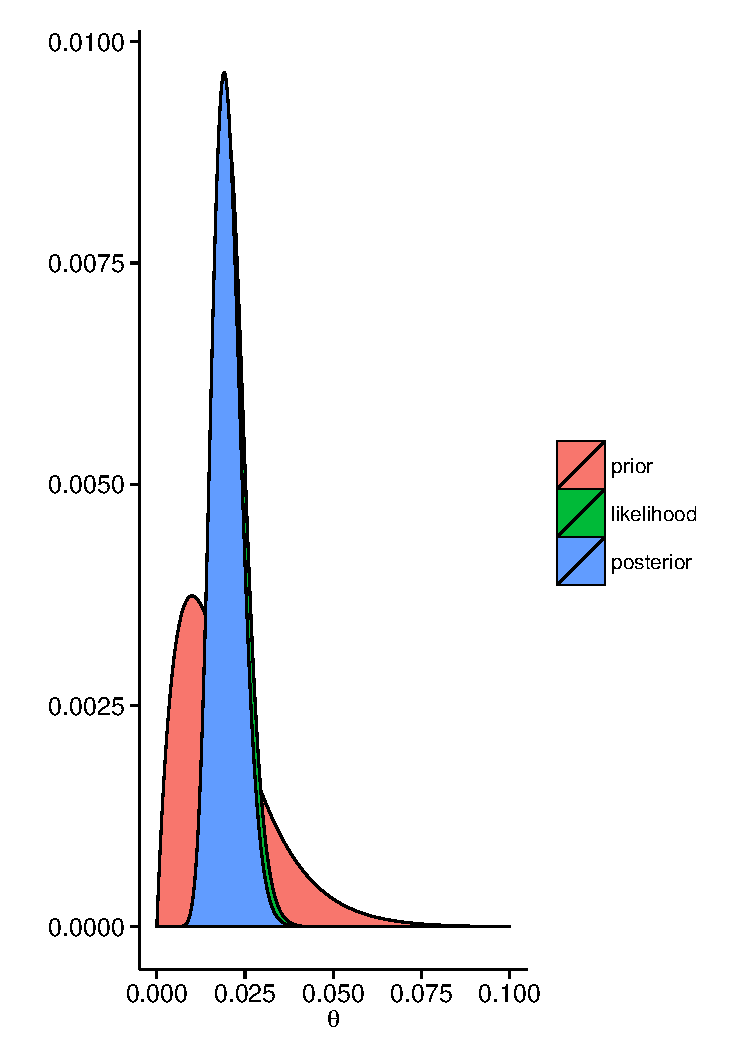
\includegraphics[scale=0.5]{bayes} 
\caption{
{ \footnotesize 
{\bf Beta prior and posterior densities plotted with a scaled likelihood resulting from a binomial model.} 
}% END: footnotesize
}
\label{fig:bayes1}
\end{figure}

Figure~\ref{fig:bayes1} shows the resulting posterior distribution along with prior and scaled likelihood.
In this case we used a fact that the beta distribution is a so called \emph{conjugate prior} for the binomial model, resulting in the posterior which is also beta-distributed and can therefore be calculated analytically.
%TODO: proof in appendix?

\subsection{Marcov Chain Monte Carlo\label{sub:MCMC}}

For every but the most trivial problems involving conjugate priors, like in our previous example, the main problem of Bayesian inference lies in the calculation of the integral in Equation~(\ref{eq:bayesian1}).
This integral leads to the marginal probability of the data $P\left(\mathbf{X}\right)$. 
For even the simplest phylogenetic problems, one has to integrate over all possible tree topologies, all of the branch lengths in those trees and all of the substitution parameters in the applied model.
Such highly-dimensional integrals are impossible to calculate analytically.
This is where the Marcov Chain Monte Carlo (MCMC) algorithms show their strength and provide a powerful method of sampling from the posterior distributions without evaluating the marginal probability.

Metropolis-Hasting algorithm, as proposed by \citet{Metropolis1953}, is an MCMC algorithm for sampling from multi-dimensional distributions.
It proceeds by constructing a Markov chain with its states being the values of the parameter of interest $\theta$ and whose equilibrium distribution is the posterior $P\left(\theta|\mathbf{X}\right)$ as defined in Equation~\ref{eq:bayesian1}.
After choosing an arbitrary starting state for the chain new candidate states $\theta^{*}$ are generated from the proposal density $q(\theta^{*} | \theta[t])$ also called the kernel.

Common choice for the kernel is to sample from a continuous uniform distribution centered around the current state of the chain, the so called jumping kernel: 

$$\theta^{*}\sim U\left[\theta[t]-\omega,\theta[t]+\omega\right],$$

\noindent
where $\omega$ is the arbitrary window size.
The chain then moves to the proposed value with probability defined by the acceptance ratio (see Equation~(\ref{eq:metropolis1})), or if the proposal is rejected the chain remains at it's current state.
The routine iterates between accept/reject steps for a specified number of times.
Both acceptance and rejection are counted as iterations od the algorithm, in fact the rejections ensure that the probabilistic properties of the target distribution are well represented in the generated sample.  
Listing in Algorithm~\ref{alg:metropolisHastings} presents the details of the Metropolis-Hastings algorithm.

\begin{algorithm}[H]
\centering
\begin{algorithmic}[1]
% \footnotesize{
%
\State Pick a starting value of the chain $\theta \left[ t \right]$ for $t=0$.
%
\For{int $\left(t=0; \; t<\text{chain length}; \; t++\right)$}
%
\State Generate a candidate state from the proposal distribution (kernel):
$$\theta^{*} \sim q(\theta[t])$$
%
\State Calculate the acceptance ratio:
$$r=\frac{prior\left(\theta^{*}\right)}{prior\left(\theta\left[t\right]\right)}\cdot\frac{Likelihood\left(\mathbf{X}|\theta^{*}\right)}{Likelihood\left(\mathbf{X}|\theta\left[t\right]\right)}\cdot\frac{q\left(\theta\left[t\right]|\theta^{*}\right)}{q\left(\theta^{*}|\theta\left[t\right]\right)}.$$
%
\State Sample $u\sim U[0,1]$.
%
\If{$\left( u < r \right)$}
%
\State Set $\theta[t+1]=\theta^*.$
%
\Else 
%
\State Set $\theta[t+1]=\theta[t].$
%
\EndIf
%
\EndFor
% }
\end{algorithmic}
\caption{
{ \footnotesize 
{\bf Metropolis-Hastings algorithm} 
}% END: footnotesize
}
\label{alg:metropolisHastings}
\end{algorithm}

We need to note several important features of the algorithm.
The most important part of the algorithm is the proposal density. 
Given the current state it proposes the next state independent of the past states.
We can recall that this is the Markov property, in fact the output of the algorithm generates a Markov chain, hence the name MCMC.
Metropolis-Hastings algorithm allows for the use of an asymetrical proposal densities such that $q\left(\theta\left[t\right]|\theta^{*}\right)\neq q\left(\theta^{*}|\theta\left[t\right]\right)$.
The acceptance probability is simply the ratio of the target posterior evaluated at the proposal and at the current state of the chain, times the ratio of the proposal: 
% prior ratio times the likelihood ratio times the proposal ratio

\begin{equation}
\frac{P\left(\theta^{*}|\mathbf{X}\right)\cdot q\left(\theta\left[t\right]|\theta^{*}\right)}{P\left(\theta\left[t\right]|\mathbf{X}\right)\cdot q\left(\theta\left[t\right]|\theta^{*}\right)}=\frac{P(\theta^{*})\cdot P\left(\mathbf{X}|\theta^{*}\right)\cdot q\left(\theta\left[t\right]|\theta^{*}\right)}{P(\theta\left[t\right])\cdot P\left(\mathbf{X}|\theta\left[t\right]\right)\cdot q\left(\theta^{*}|\theta\left[t\right]\right)}.
\label{eq:metropolis1}
\end{equation}

Note that the integral in Equation~(\ref{eq:bayesian1}) which is notoriously hard to compute cancels out in (\ref{eq:metropolis1}).
Thus to estimate the posterior $P\left(\theta|\mathbf{X}\right)$ one only needs to run the algorithm for a sufficiently long time to let the chain reach it's equilibrium, which is precisely the target posterior.

% TODO: better title, show how to derive the probabilities (in JC69 chapter)
\subsection{Example: Estimating genetic distance}

Let us revisit the toy example in which we compare two sequences and find $x=10$ differences among $n=100$ sites.
This time however we will use MCMC to estimate the genetic distance between the two sequences using Jukes and Cantor model of nucleotide substitution (see Subsection~\ref{sub:jc69}).
Genetic distance is defined as the expected number of substitutions of nucleotide base pairs per site, which to match the convention form previous sections we will denote as $\theta=rt$, where $r$ is the substitution rate (see Subsection~\ref{sub:poisson}) and $t$ is the waiting time between the two sequences.
The time and rate are as we already mentioned typically confounded, therefore they will be estimated as a single parameter of interest $\theta$.
The probability that the any descending nucleotide in a sequence is different from the ancestral nucleotide can be obtained by summing over all possible paths, between two pairs of nucleotides, i.e. $p_{ij}(t)=\underset{k\neq i}{\sum}p_{ik}(t)$.

From Equation~(\ref{eq:jc69Finite}) in Subsection~\ref{sub:jc69} we know that under the JC69 model those probabilities are all equal, therefore the probability that a single site is different between two sequences separated by distance $\theta=rt$ is given by:

\begin{equation}
p=3p_{1}\left(t\right)=\frac{3}{4}\left(1-e^{\left(-4/3\right)\theta}\right).
\label{eq:distance1}
\end{equation}

\noindent
From this we can model the likelihood of observing $x$ differences out of $n$ sites using the binomial model:

\begin{equation}
P\left(\mathbf{X}|\theta\right)=L\left(\mathbf{X}|\theta\right)=\left(\begin{array}{c}
n\\
k
\end{array}\right)p^{x}(1-p)^{n-x},
\label{eq:likelihood1}
\end{equation}

\noindent
where $p$ is as defined by Equation~(\ref{eq:distance1}).
We use an exponential prior on $\theta$ with mean $1/\lambda$:

\begin{equation}
P\left(\theta,\lambda\right)=\frac{1}{\lambda}e^{-(1/\lambda)\theta},
\label{eq:expPrior}
\end{equation}

\noindent
and set $\lambda=10$.
For the proposal we choose a uniformly distributed jumping kernel with a window size of $w=0.1$.

%---METROPOLIS PATH---%
\begin{figure}[H]
\centering
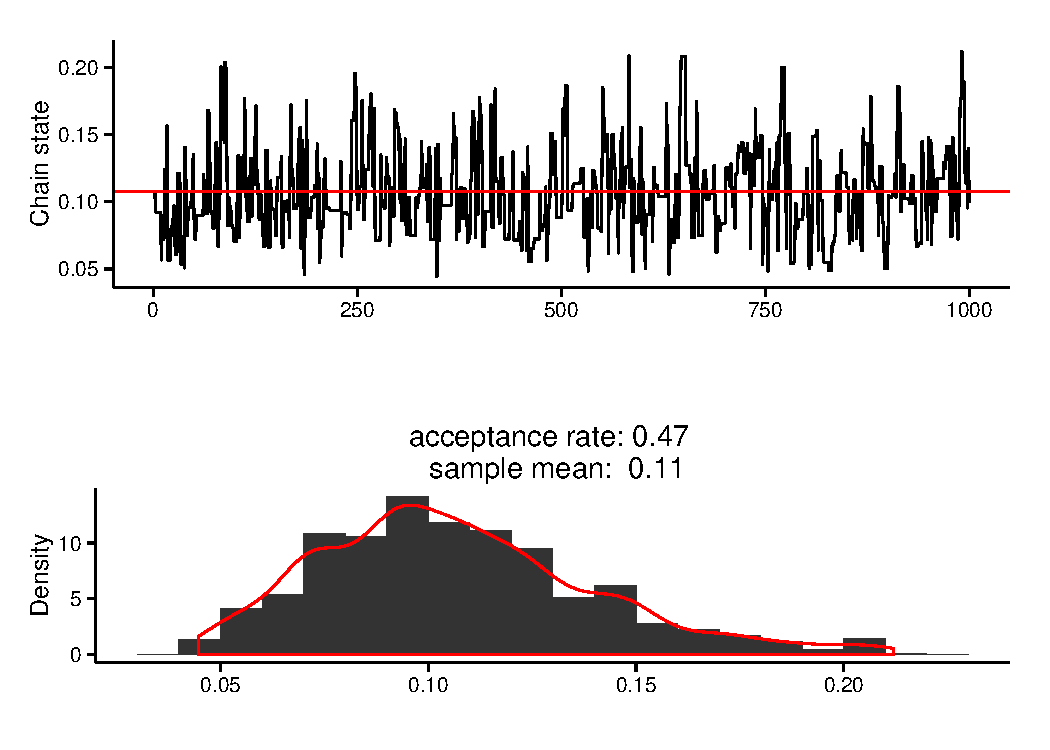
\includegraphics[scale=0.5]{metropolis} 
\caption{
{ \footnotesize 
{\bf MCMC output for estimating sequence disctance under JC69 model of nucleotide evolution..} 
}% END: footnotesize
}
\label{fig:metropolis}
\end{figure}

Figure~\ref{fig:metropolis} shows $1000$ iterations of the chain generated by Algorithm~\ref{alg:metropolisHastings} in the upper row and applied to the genetic distance problem.
The red line indicates the maximum likelihood estimate (MLE) $\hat{\theta}$ of parameter $\theta$ which is calculated by setting $\frac{d\ell\left(\mathbf{X}|\theta\right)}{d\theta}=0$, where $l\left(\mathbf{X}|\theta\right)$ is the logarithm of likelihood defined by Equation~(\ref{eq:likelihood1}):

\begin{equation}
\hat{\theta}=\frac{3}{4}log\left(1-\frac{4}{3}\cdot\frac{x}{n}\right)
\label{eq:mle}
\end{equation}

In the second row of Figure~\ref{fig:metropolis} we can see an estimate of the posterior density, along with the sample mean.
We can see that the posterior sample mean is identical to the MLE up to the second decimal place, although we have not run the chain for long.
The acceptance rate is high, suggesting that almost as many steps are accepted as are rejected.

\subsection{Bayesian phylogeography}

Phylogeography is a research direction aimed at connecting evolutionary processes, which happen over time, with the processes of spatial distribution, in actual geographical coordinates, into a joint spatio-temporal dynamic that can be used to track pathogen spread.
Historically the phylogeographical inference in molecular epidemiology ignored the reciprocal character of these two processes. 
The evolutionary relationship represented by the tree was inferred omitting the geographical information, and then the ancestral locations generated by the process of the spatial diffusion were reconstructed, conditioning on the inferred tree topology.
\citet{Lemey2009} first considered the Bayesian reconstruction that allows for joint inference of both the tree and the parameters of the spatial and temporal process that shapes the spread and evolution of 
% e.g. 
rapidly evolving viruses.
Their approach does not need to fix the tree topology, the branch lengths nor the Markov model parameters, and allows for integration over all possible values, requiring only for a specification of a prior distributions for the parameters that we aim to infer.

%TODO: plot, tree with locations
%---BAYESIAN PHYLOGENETICS TREE---%
\begin{figure}[H]
\centering
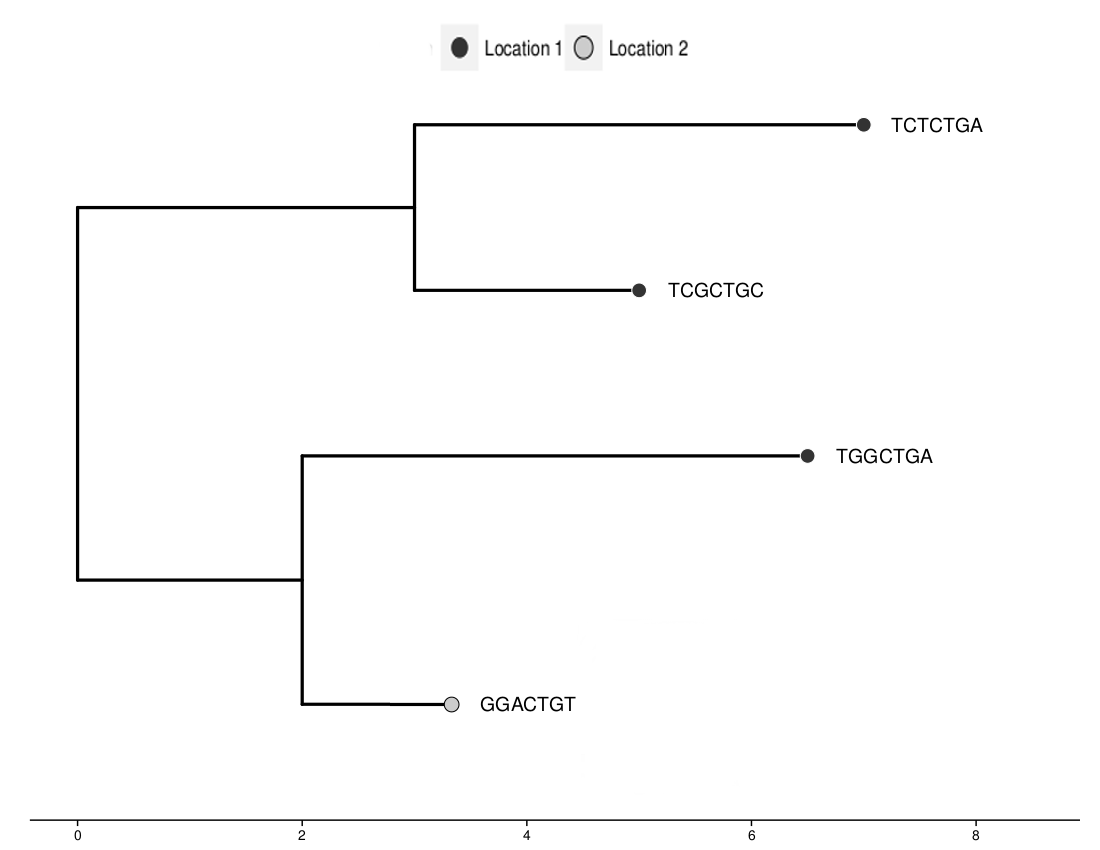
\includegraphics[scale=0.25]{phylogeotree} 
\caption{
{ \footnotesize 
{\bf Spatial location and molecular sequence data observed at the tips of a phylogenetic tree.} 
}% END: footnotesize
}
\label{fig:phylogeotree}
\end{figure}

Central to the Bayesian phylogeographic framework is the hypothesis that sequence evolution is occurring simultaneously with the process of geographical dispersal. 
The observed data, residing at the $N$ tips of phylogeny $\mathbf{F}$, is recorded as both character sequence data $\mathbf{X}=(X_{1},...,X_{N})$ and discretized geographic locations (countries, districts, cities) $\mathbf{Y}=(Y_{1},...,Y_{N})$.
We assume independent stochastic processes are responsible for generating these data, with ancestral states of $\mathbf{X}$ generated as before by a CTMC characterized by rate matrix $\mathbf{Q}$ and the unobserved ancestral locations $(Y_{N+1},...,Y_{2N-2})$ generated by a separate CTMC characterized by rate matrix $\mathbf{\Phi}$.
The entries of this matrix are the transition rates $\phi_{ij}$ between locations $i$ and $j$.
Unlike before the rate matrix does not necessarily have to be symmetrical, i.e. there exist some $i,j$ such that $\phi_{ij}\neq\phi_{ji}$.
Additionaly, a priori one would expect many of the infinitesimal rates to be zero. 
Unlike the molecular data, which is typically dense, the location data is sparse, with only one observation per taxon and many connections not observed at all.

The Bayesian framework described in Subsections~\ref{sub:bayesTheorem} and \ref{sub:MCMC} offers the unique ability to integrate different sources of information about the viruses with their genetic data, without conditioning on either one of them.
We use this ability to infer the tree topology, the ancestral spatial locations and the character substitution process giving rise to the aligned molecular sequence data. 
We assume independent stochastic processes are responsible for generating these data.
This allows us to write down the joint posterior distribution: 

% \substack{\text{aaa} \\ \text{bbb}}

\begin{eqnarray}
% \footnotesize{
P\left(\mathbf{F}, \mathbf{Q}, \mathbf{\Phi}|\mathbf{X},\mathbf{Y}\right)\propto 
\underbrace{P(\mathbf{X}|\mathbf{Q}, \mathbf{F})}_{\begin{array}{c}
\substack{\text{Sequence} \\ \text{likelihood}}
\end{array}}\cdot\underbrace{P(\mathbf{Y}|\mathbf{\Phi}, \mathbf{F})}_{\begin{array}{c}
\substack{\text{Trait} \\ \text{likelihood}}
\end{array}}\cdot
\underbrace{P(\mathbf{F})}_{\begin{array}{c}
\substack{\text{Topology} \\ \text{prior}}
\end{array}} \\ \nonumber
\cdot\underbrace{P(\mathbf{Q})}_{\begin{array}{c}
\substack{\text{Sequence substitution} \\ \text{prior}}
\end{array}}\cdot\underbrace{P(\mathbf{\Phi})}_{\begin{array}{c}
\substack{\text{Location exchange} \\ \text{prior}}
\end{array}}
% }
\label{eq:posteriorPhylogeography}
\end{eqnarray}

The likelihood component for both molecular data $\mathbf{X}$ and location data $\mathbf{Y}$ is calculated using recursive tree pruning, as described in Subsection~\ref{sub:likelihood}.
We approximate the joint posterior as written down in Equation~(\ref{eq:posteriorPhylogeography}) using MCMC methods we talked about in Subsection~\ref{sub:MCMC}.
